\chapter{Численный метод с линейными матричными неравенствами для оптимального робастного управления для систем с аддитивными неопределённостями и динамической обратной связью}\label{ch:ch5}
\section{Метод оптимального робастного управления для системы с аддитивными неопределённостями и динамической обратной связью}\label{sec:ch5/sect1}
Рассмотрим более общий случай управления с обратной связью. Вместо наблюдателя Люенбергера испльзуется регулятор с динамической обратной связью. Данный закон управления является более общим случаем управлением с обратной связью чем управление с наблюдателем Люенбергера.

Рассмотрим следующую систему:
\begin{equation}
	\label{eq:part5_linear_dynamics}
	\begin{cases}
		\dot z={A}_N {z} + {A}_r {\zeta} + {B} {u},\\
		y = {C} {N} {z} + {C} {R} {\zeta},
	\end{cases}
\end{equation}
где матрицы $A_N$,  $B$ и $C$ являются матрицами состояния, управления и наблюдения соответственно. Матрица ${A}_r$ отвечает за статическую часть матрицы состояния.

Рассмотрим следующий закон управления с динамической обратной связью:
\begin{equation}
	\label{eq:part5_controller}
	\begin{cases}
		\dot{{z}}_K = {A}_K {z}_K + {B}_K {y},\\
		{u} = {C}_K {z}_K + {D}_K {y}.
	\end{cases}
\end{equation}
Мы можем переписать предыдущие системы уравнений как:
\begin{align}
	\label{eq:part5_system1}
	&\begin{bmatrix}
		{\dot{z}} \\ {\dot{z}}_K
	\end{bmatrix}
	=
	\begin{bmatrix}
		{A}_N & 0 \\
		0 & {A}_K
	\end{bmatrix}
	\begin{bmatrix}
		{z} \\ {z}_K 
	\end{bmatrix}
	+
	\begin{bmatrix}
		{B} & 0 \\
		0 & {B}_K 
	\end{bmatrix}
	\begin{bmatrix}
		{u} \\ {y}
	\end{bmatrix}
	+
	\begin{bmatrix}
		{A}_R \\ 0 
	\end{bmatrix}
	\zeta,
	\\
	\label{eq:part5_system2}
	& \begin{bmatrix}
		{I} & -{D}_K \\
		0 & {I}
	\end{bmatrix}
	\begin{bmatrix}
		{u} \\ {y}
	\end{bmatrix}
	=
	\begin{bmatrix}
		0 & {C}_K \\
		{C} {N} & 0
	\end{bmatrix}
	\begin{bmatrix}
		{z} \\ {z}_K
	\end{bmatrix}
	+
	\begin{bmatrix}
		0 \\ {C} {R}
	\end{bmatrix}{\zeta},
\end{align}
где матрица $\bigl[ \begin{smallmatrix}  {I} & -{D}_K \\ 0 & {I} \end{smallmatrix} \bigr]$ должна быть невырожденной, которой она и будет всегда являться, следуя формуле Фробениуса \cite{froben}.
Подставим \eqref{eq:part5_system2} в \eqref{eq:part5_system1}:
\begin{align}
	\nonumber
	& \begin{bmatrix}
		{\dot{z}} \\ {\dot{z}}_K 
	\end{bmatrix}
	=\left(
	\begin{bmatrix}
		{A}_N & 0 \\
		0 & {A}_K
	\end{bmatrix}
	+
	\begin{bmatrix}
		{B} & 0 \\
		0 & {B}_K
	\end{bmatrix}
	\begin{bmatrix}
		{I} & {D}_K \\
		0 & {I}
	\end{bmatrix}
	\begin{bmatrix}
		0 & {C}_K \\
		{C}{N} & 0
	\end{bmatrix}
	\right)
	\begin{bmatrix}
		{z} \\ {z}_K
	\end{bmatrix}
	+ \\
	& + \left(
	\begin{bmatrix}
		{B} & 0 \\
		0 & {B}_K
	\end{bmatrix}
	\begin{bmatrix}
		{I} & {D}_K \\
		0 & {I}
	\end{bmatrix}
	\begin{bmatrix}
		0 \\ {C}{R}
	\end{bmatrix}
	+
	\begin{bmatrix}
		{A}_R \\ 0 
	\end{bmatrix}\right)
	{\zeta}.
\end{align}
Раскроем скобки и упростим выражение:
\begin{align}
	\label{eq:part5_cl}
	&\begin{bmatrix}
		{\dot{z}} \\ {\dot{z}}_K 
	\end{bmatrix}
	=
	\begin{bmatrix}
		{A}_N + {B}{D}_K{C}{N} & {B}{C}_K \\
		{B}_K{C}{N} &{A}_K
	\end{bmatrix}
	\begin{bmatrix}
		{z} \\ {z}_K 
	\end{bmatrix}
	+
	\begin{bmatrix}
		{A}_R + {B}{D}_K{C}{R}\\ {B}_K{C}_R
	\end{bmatrix}
	{\zeta}.
\end{align}
Обозначим:
\begin{align}
	{A}_{cl} = \begin{bmatrix}
		{A}_N + {B}{D}_K{C}{N} & {B}{C}_K \\
		{B}_K{C}{N} & {A}_K
	\end{bmatrix},
	\quad
	{z}_{cl} = \begin{bmatrix}
		{\dot{z}} \\ {\dot{z}}_K 
	\end{bmatrix},
	\quad
	{F}_{cl} = \begin{bmatrix}
		{A}_R + {B}{D}_K{C}{R}\\ {B}_K{C}_R
	\end{bmatrix}.
\end{align}
Используя новые обозначения, перепишем \eqref{eq:part5_cl}, как:
\begin{align}
	\label{eq:part5_system}
	&{\dot{z}}_{cl} = {A}_{cl} {z}_{cl}+ {F}_{cl}\zeta.
\end{align}
\begin{theorem}
	Система \eqref{eq:part5_system} асимптотически устойчива, если существуют положительно определённые матрицы ${Q}_1>0$, ${P}_1>0$, матрицы $\hat{{A}}_K$,  $\hat{{B}}_K$, $\hat{{C}}_K$ и $D_K$
	и положительный скаляр $\alpha>0$ такие, что выполняется следующие линейные матричные неравенства:
		\begin{align}\label{eq:part5_finalLMI}
		\begin{bmatrix}
			{\Theta}_1  & {A}_N + {\hat{A}}_K\T +{B}{D}_K{C}{N} & {A}_R + {B}{D}_K{C}{R}\\
			\cdots & {\Theta}_2 & {P}_{1}{A}_R + {P}_{1}{B}{D}_K{C}{R}+{P}_1{B}_K{C}{R}\\
			\cdots & \cdots & 0 
		\end{bmatrix} < 
		\begin{bmatrix}
			0 & 0\\
			0 & \alpha {I}
		\end{bmatrix},
	\end{align}
		\begin{align}\label{eq: condition}
		\begin{bmatrix} 
			{Q}_{1} & I \\ 
			I & {P}_{1}
		\end{bmatrix} > 0,
	\end{align}
	где
	\begin{align}
		{\Theta}_1 = {A}_N{Q}_{1} +{Q}_{1}{A}_N\T + {B}{\hat{C}}_K +{\hat{C}}_K\T{B}\T, \\
		{\Theta}_2 = {P}_{1}{A}_N +{A}_N\T{P}_{1}+{\hat{B}}_K{C}{N}+{N}\T{C}\T{\hat{B}}_K\T.
	\end{align}
	И коэффициенты регулятора находятся следующим образом: 
	\begin{align}
		{P}_{2} &= ({I}-{P}_{1}{Q}_{1})({Q}_{2})^{-\top},\\
		{C}_K &= ({\hat{C}}_K - {D}_K {C} {N} {Q}_{1} ) ({Q}_{2})^{-\top},\\
		{B}_K &= {P}_{2}^{-1}({\hat{B}}_K- {P}_{1}{B}{D}_K),\\
		{A}_K &= {P}_{2}^{-1}({\hat{A}}_K-{P}_{1}({A}_N+{B}{D}_K{C}{N}){Q}_{1} - {P}_{2}{B}_K{C}{N}{Q}_{1}-{P}_{1} {B}{C}_K{Q}_{2}\T)({Q}_{2})^{-\top}.
	\end{align}
\end{theorem}
\begin{proof}
	Введём кандидата в функцию Ляпунова ${V} = {z}_{cl}\T {P}{z}_{cl} > 0$ и её производную:
	\begin{align}
		{\dot{V}} = {z}_{cl}\T {P} {A}_{cl} {z}_{cl} +
		{z}_{cl}\T {A}_{cl}\T {z}_{cl} 
		+
		{z}_{cl}\T {P} {F}_{cl} {\zeta} +
		{\zeta}\T {F}_{cl}\T {z}_{cl}
		< 0,
	\end{align}
	где система считается асимптотически устойчивой в конечное время тогда и только тогда, когда существует положительно определённая матрица ${P} = \bigl[ \begin{smallmatrix}  {P}_1 & {P}_2 \\ {P}_2\T & {P}_3 \end{smallmatrix} \bigr]$.
	Производная от кандидата в функции Ляпунова может быть переписана как:
		\begin{align}
			\begin{bmatrix}
				z_{cl} \\ \zeta
			\end{bmatrix}\T
		\begin{bmatrix}
			{P} {A}_{cl} + {A}_{cl}\T {P} & {P} {F}_{cl} \\
			{F}_{cl} \T {P} & 0
		\end{bmatrix} 
		\begin{bmatrix}
			z_{cl} & \zeta
		\end{bmatrix} < 0.
	\end{align}
	Перепишем как:
	\begin{align}
		\begin{bmatrix}
			{P} {A}_{cl} + {A}_{cl}\T {P} & {P} {F}_{cl} \\
			{F}_{cl} \T {P} & 0
		\end{bmatrix} < 0.
	\end{align}
	Введём релаксацию, добавляя параметр $\alpha$, который и будет условием релаксации:
	\begin{align}\label{eq: S procedure}
		\begin{bmatrix}
			{P} {A}_{cl} + {A}_{cl}\T {P} & {P} {F}_{cl} \\
			{F}_{cl} \T {P} & 0
		\end{bmatrix} < 
		\begin{bmatrix}
			0 & 0\\
			0 & \alpha {I}
		\end{bmatrix}.
	\end{align}
	Далее необходимо избавиться от нелинейности в переменных и для этого вводим следующую лемму.
	\begin{lemma}
		Даны симметричные и невырожденные матрицы ${Q}_{1} \in \mathbb{R}^{n\times n}$ и ${P}_{1} \in \mathbb{R}^{n\times n}$. Следующие утверждения эквивалентны:\\
		
		i). Существуют симметричные и невырожденные матрицы  ${P}_{3}$ и ${Q}_{3} \in \mathbb{R}^{m\times m}$ и матрицы с полным рангом ${P}_{2}$ и ${Q}_{2} \in \mathbb{R}^{n\times m}$ такие, что
		
		\begin{align*}
			{P}=
			\begin{bmatrix} 
				{P}_{1} & {P}_{2}\\ 
				{P}_{2}\T & {P}_{3} 
			\end{bmatrix} =
			\begin{bmatrix} 
				{Q}_{1} & {Q}_{2} \\ 
				{Q}_{2}\T & {Q}_{3}
			\end{bmatrix}^{-1}={Q}^{-1}>0,
		\end{align*} 
		где ${Q}_{CL}=
		\begin{bmatrix} 
			{Q}_{1} & {I} \\ {Q}_{2}\T & 0
		\end{bmatrix}$ является матрицей полного ранга.\\
		
		ii). \begin{align*}
			\begin{bmatrix} 
				{Q}_{1} & I \\ 
				I & {P}_{1}
			\end{bmatrix} > 0.
		\end{align*}
	\end{lemma}
	\begin{proof}
		Из i)., берём 
		\begin{align}
			&{P} = {Q}^{-1},\\
			&{P}{Q}={I},\\
			&\begin{bmatrix} 
				{P}_{1} & {P}_{2}\\ 
				{P}_{2}\T & {P}_{3} 
			\end{bmatrix}
			\begin{bmatrix} 
				{Q}_{1} & {Q}_{2} \\ 
				{Q}_{2}\T & {Q}_{3}
			\end{bmatrix} = 
			\begin{bmatrix}
				{I} & 0 \\
				0 & {I}
			\end{bmatrix}.
		\end{align}
		Раскрыв скобки в последнем уравнении, получаем:
		\begin{align}
			&{P}_{1}{Q}_{1}+{P}_{2}{Q}_{2}\T ={I},\\
			&{P}_{1}\T{Q}_{2}+{P}_{2}{Q}_{3} =0\label{eq: lemma mult1},\\
			&{P}_{2}\T{Q}_{1}+{P}_{3}{Q}_{2}\T=0,\\
			&{P}_{2}\T{Q}_{2}+{P}_{3}{Q}_{3}= {I} \label{eq: lemma mult2}.
		\end{align}
		Из данных уравнений получаем:
		\begin{align}
			{P}{Q}_{CL}={P}_{CL},
		\end{align}
		где
		\begin{align}
			{Q}_{CL}=
			\begin{bmatrix}
				{Q}_{1} & {I}\\
				{Q}_{2}\T & 0
			\end{bmatrix},\\
			{P}_{CL}=
			\begin{bmatrix}
				{I} & {P}_{1} \\
				0 & {P}_{2}\T
			\end{bmatrix}.
		\end{align}
		Матрица ${Q}_{2}$ имеет полный ранг, и матрица ${Q}_{CL}$ тоже имеет полный ранг, тогда
		\begin{align}
			0<{Q}_{CL}\T {P} {Q}_{CL} = {Q}_{CL}\T {P}_{CL} = 
			\begin{bmatrix} 
				{Q}_{1} & I \\ 
				I & {P}_{1}
			\end{bmatrix}.
		\end{align}
		
		И наоборот, предположим ii). верно. Мы можем умножить на минус $1$ и применить дополнение Шура к неравенству 
		$\bigl( \begin{smallmatrix} 
			{Q}_{1} & I \\ 
			I & {P}_{1}\end{smallmatrix} \bigr) <0$. 
		И тогда, согласно дополнению Шура, получаем $-{P}_{1}<0$ и $-{Q}_{1}-(-{I})(-{P}_{1})^{-1}(-{I})\T<0$. Упрощая, избавляясь от матриц тождества, мы получаем ${P}_{1}^{-1}-{Q}_{1}<0$, и она имеет полный ранг, то есть можно найти обратную матрицу. Что также означает, что ${I}-{P}_{1}{Q}_{1}$ имеет обратную матрицу.
		
		Выбираем любые две матрицы полного ранга ${P}_{2}$ и ${Q}_{2}$, такие что ${P}_{2}{Q}_{2}\T={I}-{P}_{1}{Q}_{1}$. И поскольку ${P}_2$ и ${Q}_2$ имеют полный ранг, ${Q}_{CL}=\bigl[\begin{smallmatrix}  
			{Q}_{1} & {I}\\
			{Q}_{2}\T & 0
		\end{smallmatrix} \bigr]$ и 
		${P}_{CL}=\bigl[ \begin{smallmatrix}
			{I} & {P}_{1} \\
			0 & {P}_{2}\T
		\end{smallmatrix} \bigr]$ также имеют полный ранг и существуют обратные матрицы к ним.
		
		Обозначим ${P}$ и ${Q}$ как 
		\begin{align*}
			{P} = {P}_{CL}{Q}_{CL}^{-1}, \qquad {Q} ={Q}_{CL}{P}_{CL}^{-1}.
		\end{align*} 
		Далее перемножая ${P}$ и ${Q}$, мы получаем единичную матрицу
		\begin{align*}
			{P}{Q}={P}_{CL}{Q}_{CL}^{-1}{Q}_{CL}{P}_{CL}^{-1}={I}.
		\end{align*}
		Таким образом ${P}={Q}^{-1}$.
		
		${P}_3$ и ${Q}_3$ при необходимости можно найти из \eqref{eq: lemma mult1}--\eqref{eq: lemma mult2}.
	\end{proof}
	Домножим с правой и левой стороны неравенство (\ref{eq: S procedure}) на матрицы $diag({Q}_{CL}\T, {I}, {I})$ и $diag({Q}_{CL}, {I}, {I})$ для линейной независимости в переменных:
	\begin{align}
		\begin{bmatrix}
			{Q}_{CL}\T{A}_{CL}\T {P}_{CL} + {P}_{CL}\T{A}_{CL}{Q}_{CL} & {P}_{CL}\T{F}_{CL} \\
			{F}_{CL}\T{P}_{CL} & 0
		\end{bmatrix} < 
		\begin{bmatrix}
			0 & 0\\
			0 & \alpha {I}
		\end{bmatrix}.
	\end{align}
	Далее мы постепенно раскрываем и упрощаем каждый компонент уравнения:
	\begin{align}
		{P}_{CL}\T{F}_{CL} = \begin{bmatrix}
			{I} & 0 \\
			{P}_{1} & {P}_{2}
		\end{bmatrix}
		\begin{bmatrix}
			{A}_R + {B}{D}_K{C}{R}\\ {B}_K{C}_R
		\end{bmatrix} =
		\begin{bmatrix}
			{A}_R + {B}{D}_K{C}{R}\\
			{P}_{1}{A}_R + {P}_{1}{B}{D}_K{C}{R}+{P}_1{B}_K{C}{R}
		\end{bmatrix},
	\end{align}
	%
	\begin{align}
		&{Q}_{CL}\T{A}_{CL}\T {P}_{CL} + {P}_{CL}\T{A}_{CL}{Q}_{CL} = \nonumber \\
		& = \begin{bmatrix}
			{A}_N{Q}_{1} +{Q}_{1}{A}_N\T + {B}{\hat{C}}_K +{\hat{C}}_K\T{B}\T & {A}_N + {\hat{A}}_K\T +{B}{D}_K{C}{N}\\
			{A}_N\T + {N}\T{C}\T{D}_K\T{B}\T+{\hat{A}}_K & {P}_{1}{A}_N +{A}_N\T{P}_{1}+{\hat{B}}_K{C}{N}+{N}\T{C}\T{\hat{B}}_K\T
		\end{bmatrix},   
	\end{align}
	\begin{align}
		&{\hat{C}}_K= {D}_K{C}{N}{Q}_{1} + {C}_K{Q}_{2}\T,\\
		&{\hat{B}}_K = {P}_{1}{B}{D}_K + {P}_{2}{B}_K,\\
		&{\hat{A}}_K = {P}_{1}({A}_N+{B}{D}_K{C}{N}){Q}_{1}+{P}_{2}{B}_K{C}{N}{Q}_{1}+{P}_{1}{B}{C}_K{Q}_{2}\T+{P}_{2}{A}_K{Q}_{2}\T.
	\end{align}
	Финальное неравенство
	\begin{align}\label{eq: final LMI}
		\begin{bmatrix}
			{\Theta}_1  & {A}_N + {\hat{A}}_K\T +{B}{D}_K{C}{N} & {A}_R + {B}{D}_K{C}{R}\\
			\cdots & {\Theta}_2 & {P}_{1}{A}_R + {P}_{1}{B}{D}_K{C}{R}+{P}_1{B}_K{C}{R}\\
			\cdots & \cdots & 0 
		\end{bmatrix} < 
		\begin{bmatrix}
			0 & 0\\
			0 & \alpha {I}
		\end{bmatrix},
	\end{align}
	где
	\begin{align}
		&{\Theta}_1 = {A}_N{Q}_{1} +{Q}_{1}{A}_N\T + {B}{\hat{C}}_K +{\hat{C}}_K\T{B}\T, \\
		&{\Theta}_2 = {P}_{1}{A}_N +{A}_N\T{P}_{1}+{\hat{B}}_K{C}{N}+{N}\T{C}\T{\hat{B}}_K\T.
	\end{align}
	И держится неравенство: 
	\begin{align}\label{eq: condition}
		\begin{bmatrix} 
			{Q}_{1} & I \\ 
			I & {P}_{1}
		\end{bmatrix} > 0.
	\end{align}
	Это и является линейным матричным неравенством с переменными ${Q}_1, {P}_1, {\hat{A}}_K, {\hat{B}}_K,{\hat{C}}_K, {D}_K$ и $\alpha$.
\end{proof}
Целевой функцией будет являться минимизация переменных матриц. Оптимизационная задача будет выглядеть следующим образом:
%
\begin{equation}
	\label{eq:thm2_OCP}
	\begin{aligned}
		& \underset{{Q}_1,{P}_1, {\hat{A}}_K, {\hat{B}}_K,{\hat{C}}_K, {D}_K, \alpha }{\text{минимизируя}}
		& &\operatorname{tr}({Q}_1\T{W}_q{Q}_1)+ \operatorname{tr}({P}_1\T{W}_p{P}_1) \\
		& \text{при ограничениях}
		& & \begin{cases}
			\text{условия \eqref{eq: final LMI}, \eqref{eq: condition}},
		\end{cases}
	\end{aligned}
\end{equation}
где ${W}_q$ и ${W}_p$ --- весовые матрицы.

\section{Пример применения метода оптимального робастного управления для системы с аддитивной неопределённостью и динамической обратной связью}\label{sec:ch5/sect2}

Для демонстрации работы численного метода используется комплекс программ, описанный в разделе \ref{sec:ch3/sect3/sub1} и входные данные, описанные в разделе \ref{sec:ch3/sect3/sub2}.

Решим следующую ЗОУ \eqref{eq:thm2_OCP}.
%
На рисунке \ref{fig:output_cost} изображён график зависимости значения целевой функции от значения параметра $\alpha$. 
\begin{figure}[ht]
	\centerfloat{
		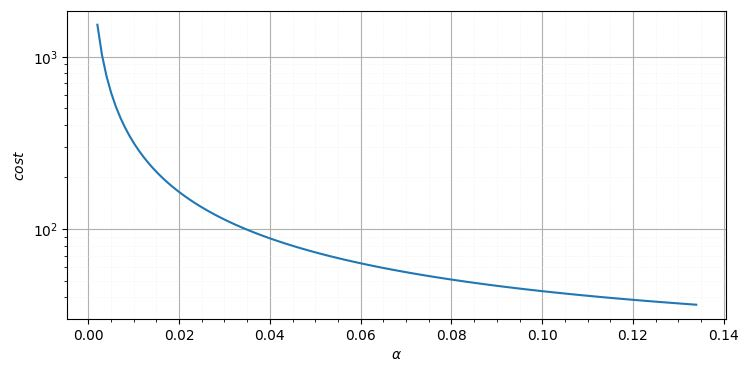
\includegraphics[scale=1.2]{images/output_cost.JPG}
	}
	\caption{Целевая функция для ЗОУ \eqref{eq:thm2_OCP}, решённой для плоского четвероногого робота, построенная относительно параметра $\alpha$; вертикальная ось масштабирована логарифмически, обе оси без единиц.} \label{fig:output_cost}
\end{figure}
Данный график показывает, что у ЗОУ есть решения и можно выбрать оптимальное значение параметра $\alpha$.
 
\begin{figure}[ht]
	\centerfloat{
		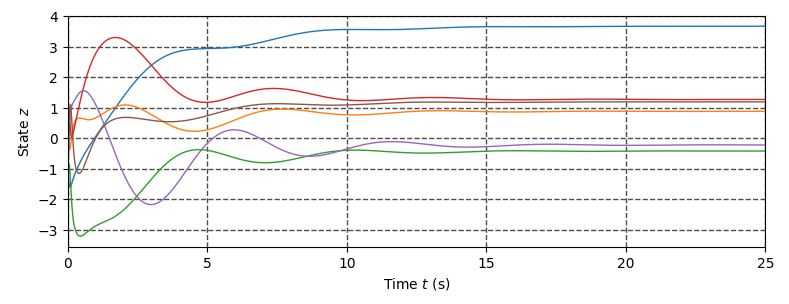
\includegraphics[scale=1.2]{images/output_state_z.JPG}
	}
	\caption{Вектор состояния от времени при решении \eqref{eq:thm2_OCP} для плоского четвероногого робота.} \label{fig:output_state_z}
\end{figure}
На рисунке \ref{fig:output_state_z} показан график зависимости вектора состояния при решении проблемы \eqref{eq:thm2_OCP} для заданных случайных начальных условий и временном промежутке в 25 секунд.

\begin{figure}[ht]
	\centerfloat{
		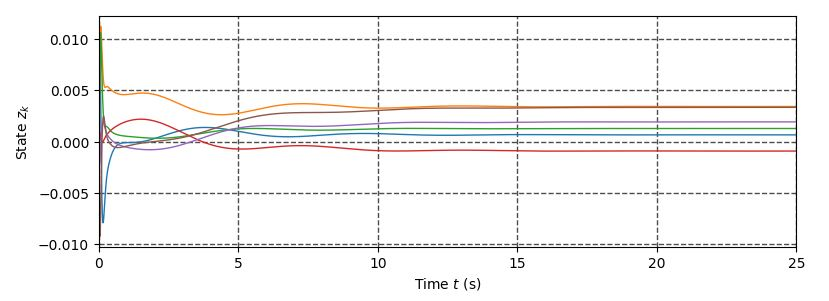
\includegraphics[scale=1.2]{images/output_state_zk.JPG}
	}
	\caption{Вектор состояния регулятора от времени при решении \eqref{eq:thm2_OCP} для плоского четвероногого робота.} \label{fig:output_state_zk}
\end{figure}

На рисунке \ref{fig:output_state_zk} показан график зависимости вектора состояния регулятора при решении проблемы \eqref{eq:thm2_OCP} для заданных случайных начальных условий и временном промежутке в 25 секунд. Из вышеуказанных графиков векторов состояния от времени можно отметить, что система с динамической обратной связью стабилизируется.